\documentclass{article}
\usepackage{tikz}
\usepackage[a4paper]{geometry}
\usepackage{fancyhdr}
\pagestyle{fancy}
\lhead{Magnetfelder}
\rhead{September 2025}
\begin{document}
\section{Magnetfelder}
Ein jeder Magnet hat zwei Pole; einen \emph{Nord-} und einen \emph{Südpol}. Ähnlich wie bei der Ladung, ist es auch hier so, dass sich gleinamige Pole abstoßen, ungleichnamige Pole ziehen sich an. \newline  
Um einen jeden Magneten existiert ein Magnetfeld, dargestellt durch geschlossene Feldlinien, welche von Nord nach Süd gehen. Weil der magnetische Nordpol eines Kompass sich zum geographischen Nordpol der Erde, welcher eigentlich der magnetische Südpol ist, dreht, folgt dass sich eine Kompassnadel entlang der Feldlinien eines Magnetfeldes ausrichtet. \newline 
 
\subsection{Magnetfeldlinien}
\begin{minipage}{\dimexpr\linewidth-3cm} 
 Darüberhinaus hat auch jeder stromdurchflossene Leiter ein eigenes Magnetfeld, welches mithilfe der linken Hand bestimmt werden kann. Zeigt der Daumen von der linken Hand in die Richtung, in welche sich die Elektronen bewegen, so zeigen die anderen Finger, wenn sie zusammengezogen werden, in die Richtung der Feldlinien. \newline
 Die Magnetfeldlinien einer Spule sind so ausgerichtet, dass wenn die Finger der linken Hand in Richtung der Windung zusammengezogen werden, der Daumen in Richtung der Magnetfeldlinien innerhalb der Spule zeigt. Größer gedacht, inklusive des Leiters, welcher über die Windungen hinaus geht, kann es sich auch so vorgestellt werden, dass der Nordpol auf der negativen Seite ist.
\end{minipage}
\hfill
\begin{minipage}{3cm}
 \center
 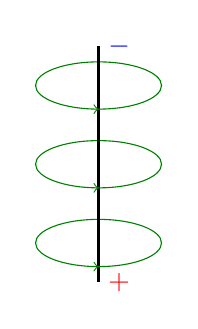
\begin{tikzpicture}
  \draw (0, 0) node[blue, right] {$-$};
  \draw (0, -3) node[red, right] {$+$};
 
  \foreach \y in {-2.5,...,-0.5} { 
    \begin{scope}
     \clip (-0.9,\y+0.5) rectangle (0.9,\y);
     \draw[green!50!black] (0, \y) ellipse (0.8cm and 0.3cm);
    \end{scope} 
  }  
 
  \draw[thick] (0, 0) -- (0, -3);
 
  \foreach \y in {-2.5,...,-0.5} { 
    \begin{scope}
     \clip (-0.9,\y) rectangle (0.9,\y-0.5);
     \draw[green!50!black] (0, \y) ellipse (0.8cm and 0.3cm);
     \draw[green!50!black, ->] (-0.01, \y-0.3) -- (0, \y-0.3);
    \end{scope} 
  } 
 \end{tikzpicture} 
\end{minipage} 
 
\end{document}